\section{Dataføder: SPI og SD-kort}\fixme{andet ordvalg}

En oversigt over funktionsfordelingen\fixme{andet ordvalg} i
dataføreren\fixme{andet ordvalg} kan ses i
figur\vref{fig:software-spi-sd-oversigt}.

\begin{figure}[htbp]
  \centering
  \includegraphics[width=\textwidth]{../brugere/kjaergaard/datafeeder-oversigt}
  \caption{Diagram over funktionsfordeling i dataføderen.}
  \label{fig:software-spi-sd-oversigt}
\end{figure}

Kommunikationen med SD-kortet foregår gennem SPI'en.\fixme{afsnit skal
  skrives færdig}. En eksempel på en forespørgsel med tilhørende svar
kan ses i figur\vref{fig:software-spi-sd-handling}

\begin{figure}[htbp]
  \centering
  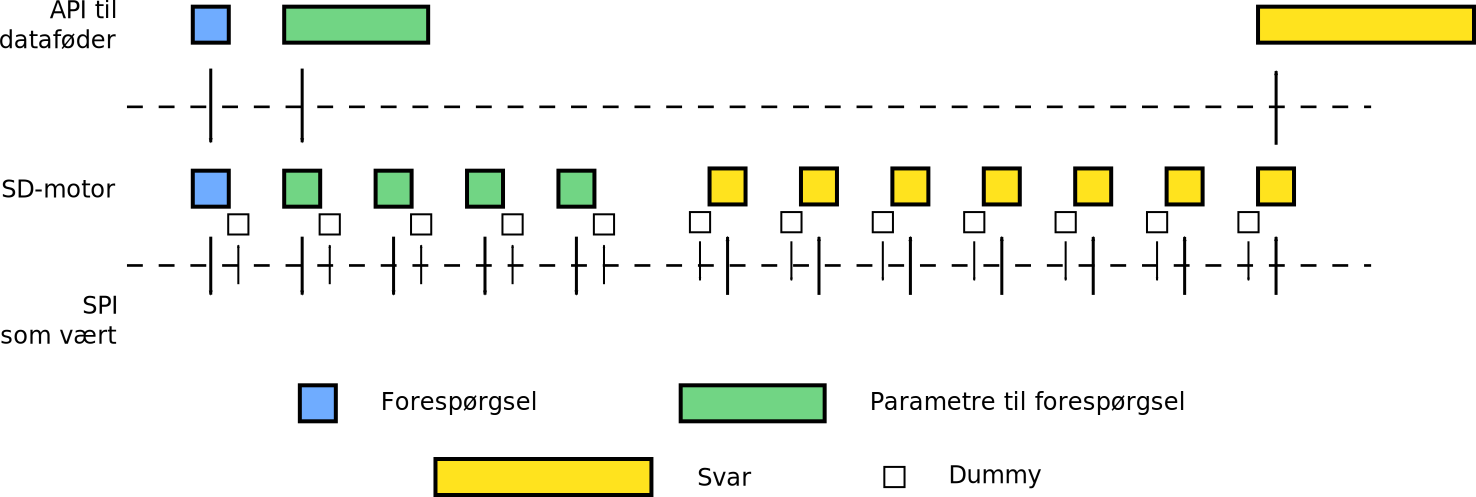
\includegraphics[width=\textwidth]{../brugere/kjaergaard/datafeeder-handling}
  \caption{Handlingdiagram ved kommunikation med SD-kortet.}
  \label{fig:software-spi-sd-handling}
\end{figure}

%%% Local Variables: 
%%% mode: latex
%%% TeX-master: "../master"
%%% End: 